\chapter{RNA Seq}

\section{软件的安装}
主要使用到了cutadapt、STAR、fastqc、stringtie,首先使用在conda config中添加bioconda,再创建一个环境,添加会使用到的各种包。
\begin{lstlisting}
    conda config --add channels bioconda
    conda create -n rnaseq
    conda activate rnaseq
    conda install cutadapt STAR fastqc stringtie
\end{lstlisting}

\begin{figure}[ht]
    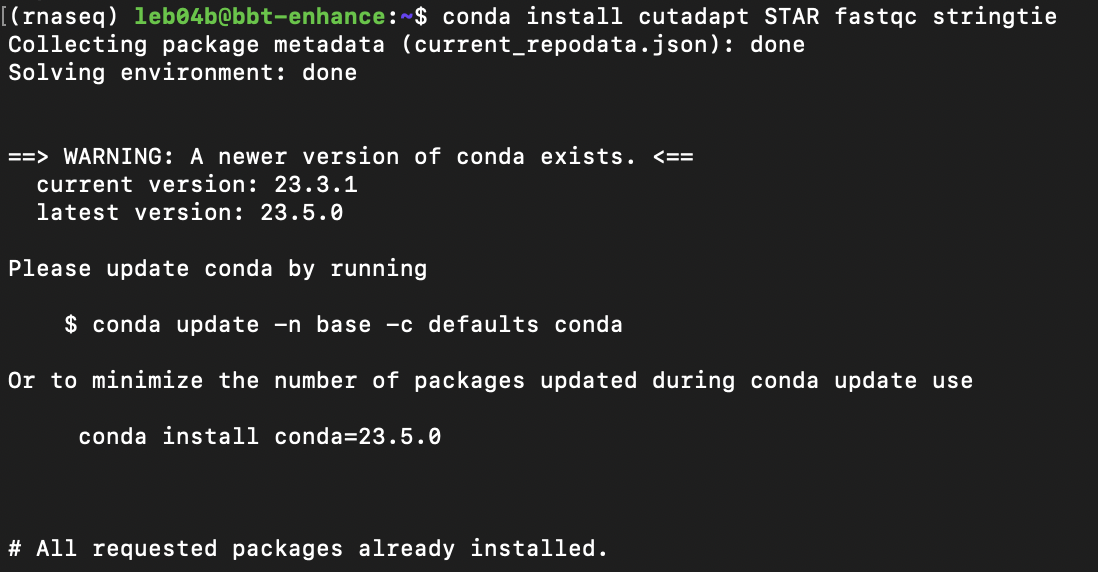
\includegraphics[width=13cm]{image/rnaseq/package.PNG}
\end{figure}

\section{RNA-seq上游分析}
RNA-seq上游分析与ChIP-Seq类似,参见。故此处仅简单提及。

\subsection{质控}
原始数据为fastq.qz文件,一般是双端配套的比对结果,有两个文件
使用fastqc进行质控,最后得到两个文件,其中一个为html文件,可用网页浏览,也可以在VSCode中安装html插件查看。

\begin{figure}[ht]
    \begin{minipage}[C]{0.9\textwidth}
        \centering
        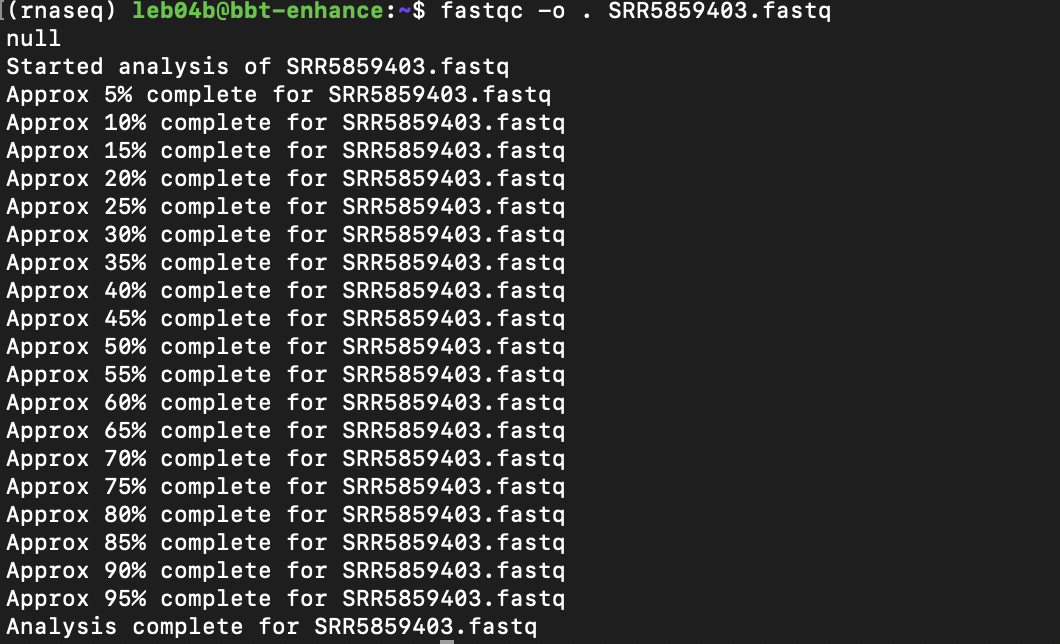
\includegraphics[width=13cm]{image/rnaseq/qc.PNG}
    \end{minipage}

    \begin{minipage}[C]{0.9\textwidth}
        \centering
        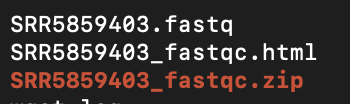
\includegraphics[width=5cm]{image/rnaseq/qcfile.PNG}
    \end{minipage}
\end{figure}

\subsection{使用cutadapt去接头}

\subsection{比对}
下载参考基因组,star建立索引。比对后,可以得到bam、log、log out、log final out文件

\subsection{定量}
使用stringtie,输入bam文件,得到gtf文件(包含基因、数量)

使用stringtie的自带脚本prepDE.py运行得到的gtf文件得到表达矩阵csv文件

\section{RNA-seq下游分析}
表达矩阵每一列是一个样本,每一行是一个基因。(注意基因 symbol 和ensembl id 的转换)

clusterprofiler包中的bitr函数可以进行symbol到ensembl id的转化

\subsubsection{差异表达基因分析(在R的环境下运行)}

引入相应的包
\begin{lstlisting}
    library(tidyverse)
    library(pheatmap)
    library(DESeq2)
    library(readxl)
    library(EnhancedVolcano)
    library(clusterProfiler)
    library(org.Hs.eg.db)

    #加载常用的包
    #如未下载,可使用类似代码进行安装
    #
    #if (!require("BiocManager", quietly = TRUE))
    #  install.packages("BiocManager")
    #BiocManager::install("EnhancedVolcano")
    #安装后,必须使用library命令激活

\begin{lstlisting}
    getwd()
    setwd('leb/rnaseq')
    #切换工作目录
\end{lstlisting}

读取生成的文件
\begin{lstlisting}
    rna_seq <- read_excel(
    "RNAseq.xlsx",
    sheet = "Readcounts"
    )
    #读入excel文件
    #注意!数据类型未tibble,不是data.frame!
\end{lstlisting}

进行id转化
\begin{lstlisting}
    genid <- bitr(rna_seq$Geneid, fromType = "ENSEMBL", toType = "SYMBOL",
        OrgDb = org.Hs.eg.db)
        # org.Hs.eg.db是一个homo sapiens数据库,根据该数据库中的注释进行id转换

\end{lstlisting}

整理数据格式
\begin{lstlisting}
    rna_seq <- rna_seq %>%
    mutate(Gene = ...1) %>%
    dplyr::select(-...1) %>%
    group_by(Gene) %>%
    summarise_all(sum) %>% # 这里的sum是对每一列进行求和,其实这个矩阵应该是已经整理好的不用。
    as.data.frame()

    # 使用管道符

    rownames(rna_seq) <- rna_seq$Gene
    rna_seq <- rna_seq[, -1] # remove Gene column
    print(head(rna_seq))
    rna_seq <- rna_seq[-c(1:20), ] # 去掉前20行,这里面是一些不是基因的东西
    rna_seq <- rna_seq[rowSums(rna_seq) >= 10, ] # 去掉在所有样本里面表达量小于10的基因
\end{lstlisting}

直接生成图片的时候要把plot框调到合适大小
\begin{lstlisting}
    > biplot(p)
    Error in grid.Call(C_convert, x, as.integer(whatfrom), as.integer(whatto),  :
    Viewport has zero dimension(s)
\end{lstlisting}

\subsubsection{数据质控}
Plotcount 可以查看目标基因的表达情况
\begin{lstlisting}
    plotCounts(dds, gene = "RBMX", intgroup = "type")
\end{lstlisting}

\begin{figure}[ht]
    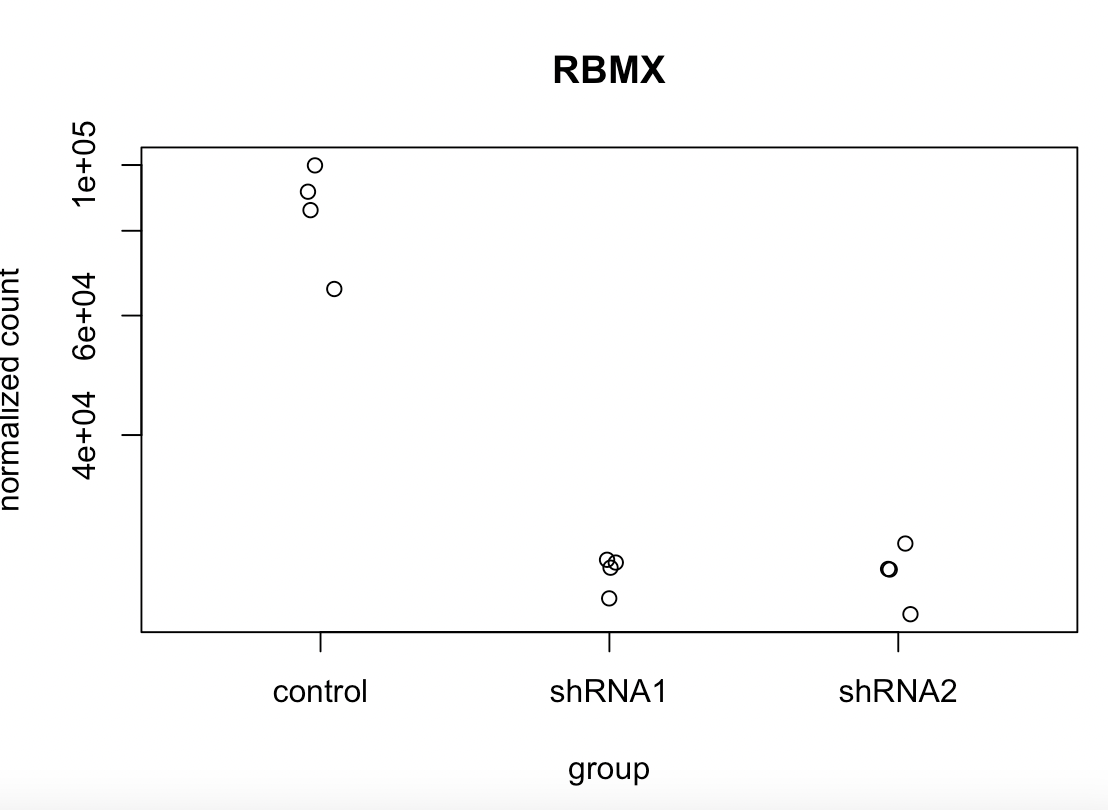
\includegraphics[width=10cm]{image/rnaseq/qc2.png}
\end{figure}

使用PCA降维聚类
\begin{lstlisting}
    library(PCAtools)
    vst <- rna_seq
    meta <- data.frame(row.names = colnames(rna_seq), type = id$type)
    p <- pca(vst, metadata=meta, removeVar = 0.05)
    biplot(p)
\end{lstlisting}

\begin{figure}[ht]
    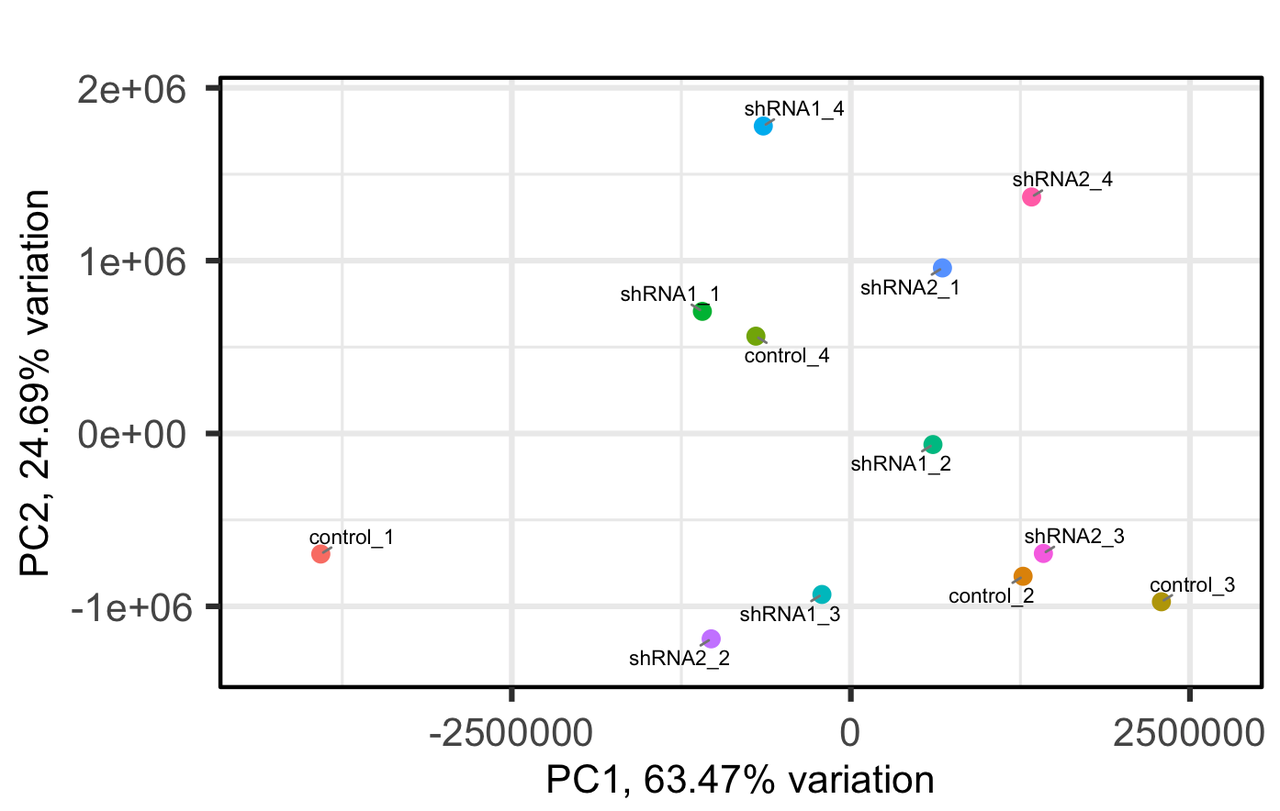
\includegraphics[width=13cm]{image/rnaseq/pca.png}
\end{figure}

火山图的绘制,如图\ref{volcano}。
\begin{lstlisting}
    res1 <- results(dds, name="type_shRNA1_vs_control")
    res2 <- results(dds, name="type_shRNA2_vs_control")
    EnhancedVolcano(res1,
    lab = rownames(res1),
    x = "log2FoldChange",
    y = "pvalue"
    )
    EnhancedVolcano(res2,
    lab = rownames(res2),
    x = "log2FoldChange",
    y = "pvalue"
    )
\end{lstlisting}

\begin{figure}[ht]
    \centering
    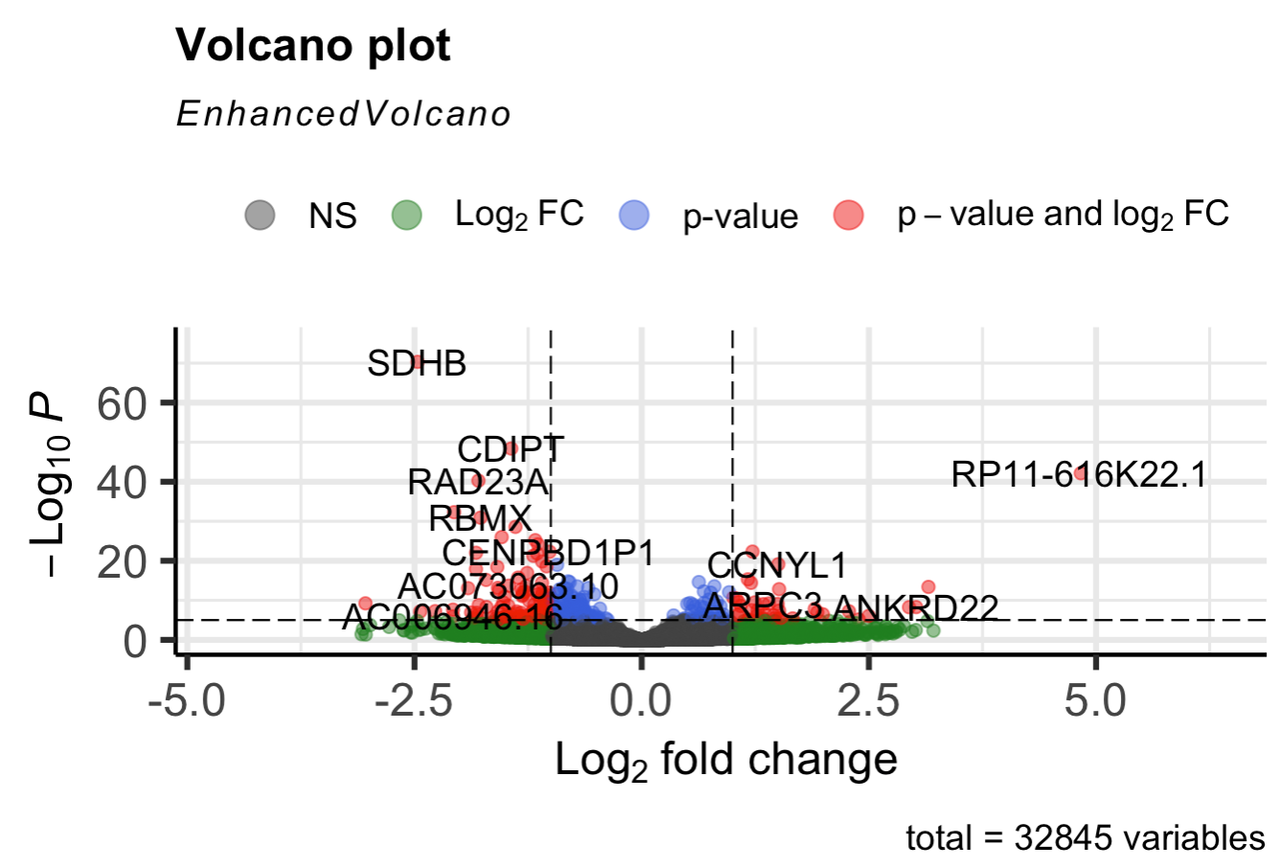
\includegraphics[width=13cm]{image/rnaseq/volcano.png}
    \caption{火山图}
    \label{volcano}
\end{figure}

pheatmap对差异基因绘制热图,如图\ref{dif}。
\begin{lstlisting}
    res_filtered <- res2 %>%
    as.data.frame() %>%
    rownames_to_column("Gene") %>%
    filter(padj < 0.05 & abs(log2FoldChange) > 1)
    dim(res_filtered)
    print(head(res_filtered))
    differential_genes <- res_filtered$Gene
    diff_matrix <- rna_seq[sample(differential_genes, 50), ]
    RBMX <- rna_seq["RBMX",]
    diff_matrix <- rbind(diff_matrix, RBMX)
    pheatmap(diff_matrix, scale = "row")
    ggsave("heatmap.png", width = 10, height = 10)
\end{lstlisting}

\begin{figure}[ht]
    \centering
    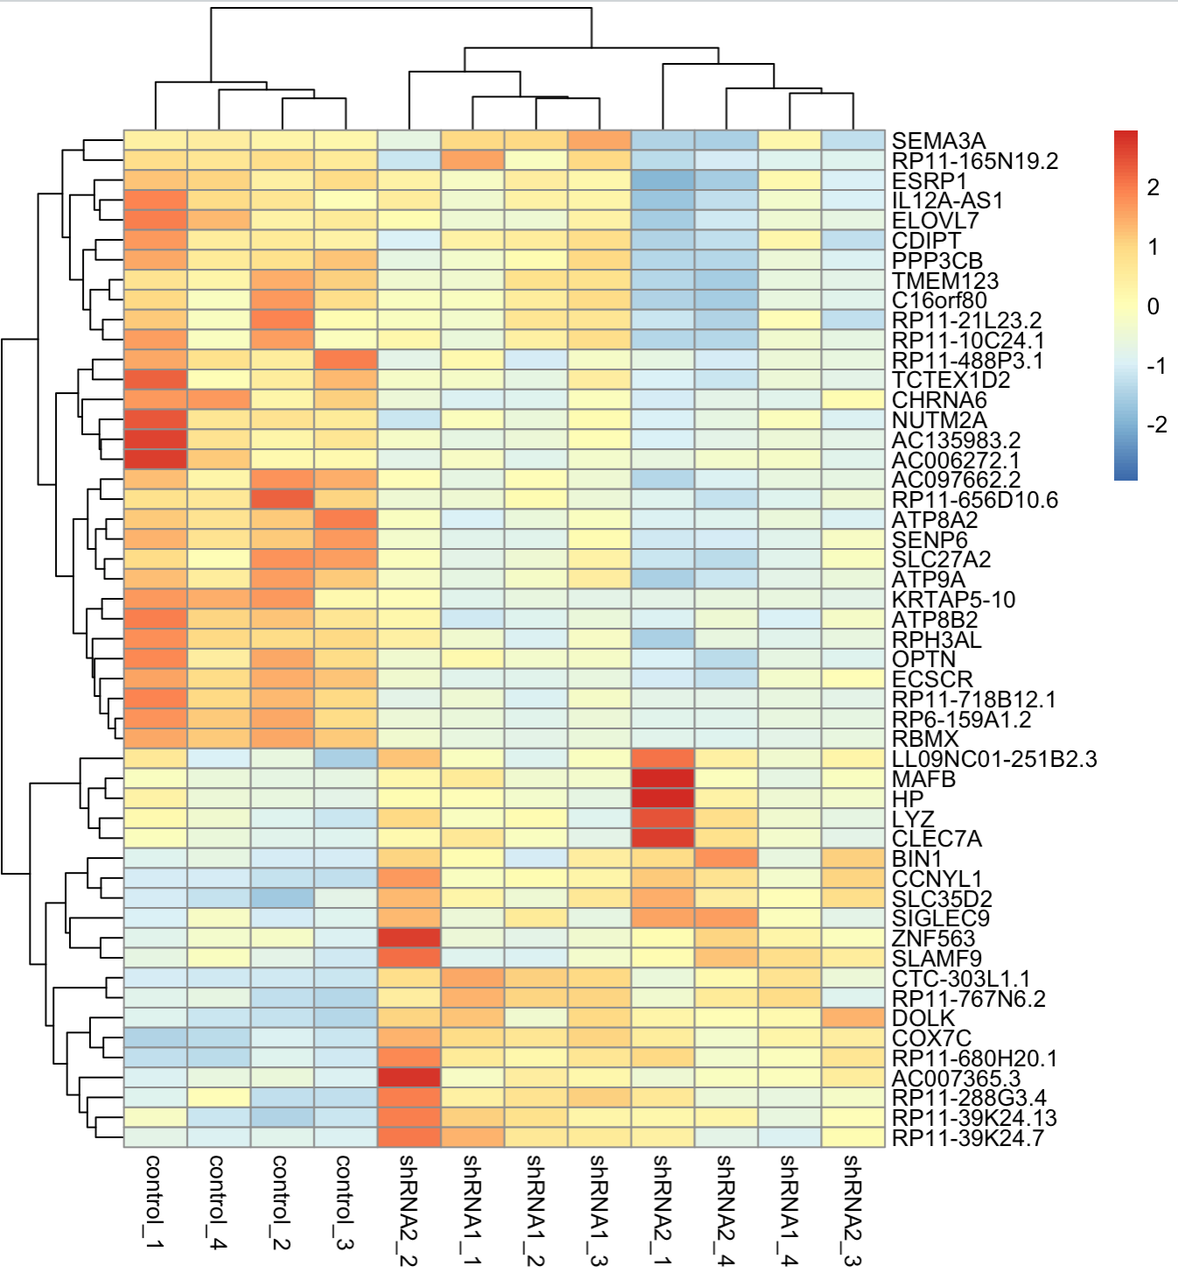
\includegraphics[width=10cm]{image/rnaseq/heatmap.png}
    \caption{基因差异表达结果}
    \label{dif}
\end{figure}

\subsubsection{GO富集分析}
使用clusterprofile包可以进行go富集分析,如图\ref{go}。
\begin{lstlisting}
    library(clusterProfiler)
    library(org.Hs.eg.db)
    #gene ontology
    go_bp <- enrichGO(gene = differential_genes,
    OrgDb = org.Hs.eg.db,
    keyType = "SYMBOL",
    ont = "BP", # BP: biological process, MF: molecular function, CC: celluar component, ALL
    pAdjustMethod = "BH",
    pvalueCutoff = 0.05,
    qvalueCutoff = 0.05)
    dotplot(go_bp, title = "GO Biological Pathway", showCategory = 10)
\end{lstlisting}

\begin{figure}[ht]
    \centering
    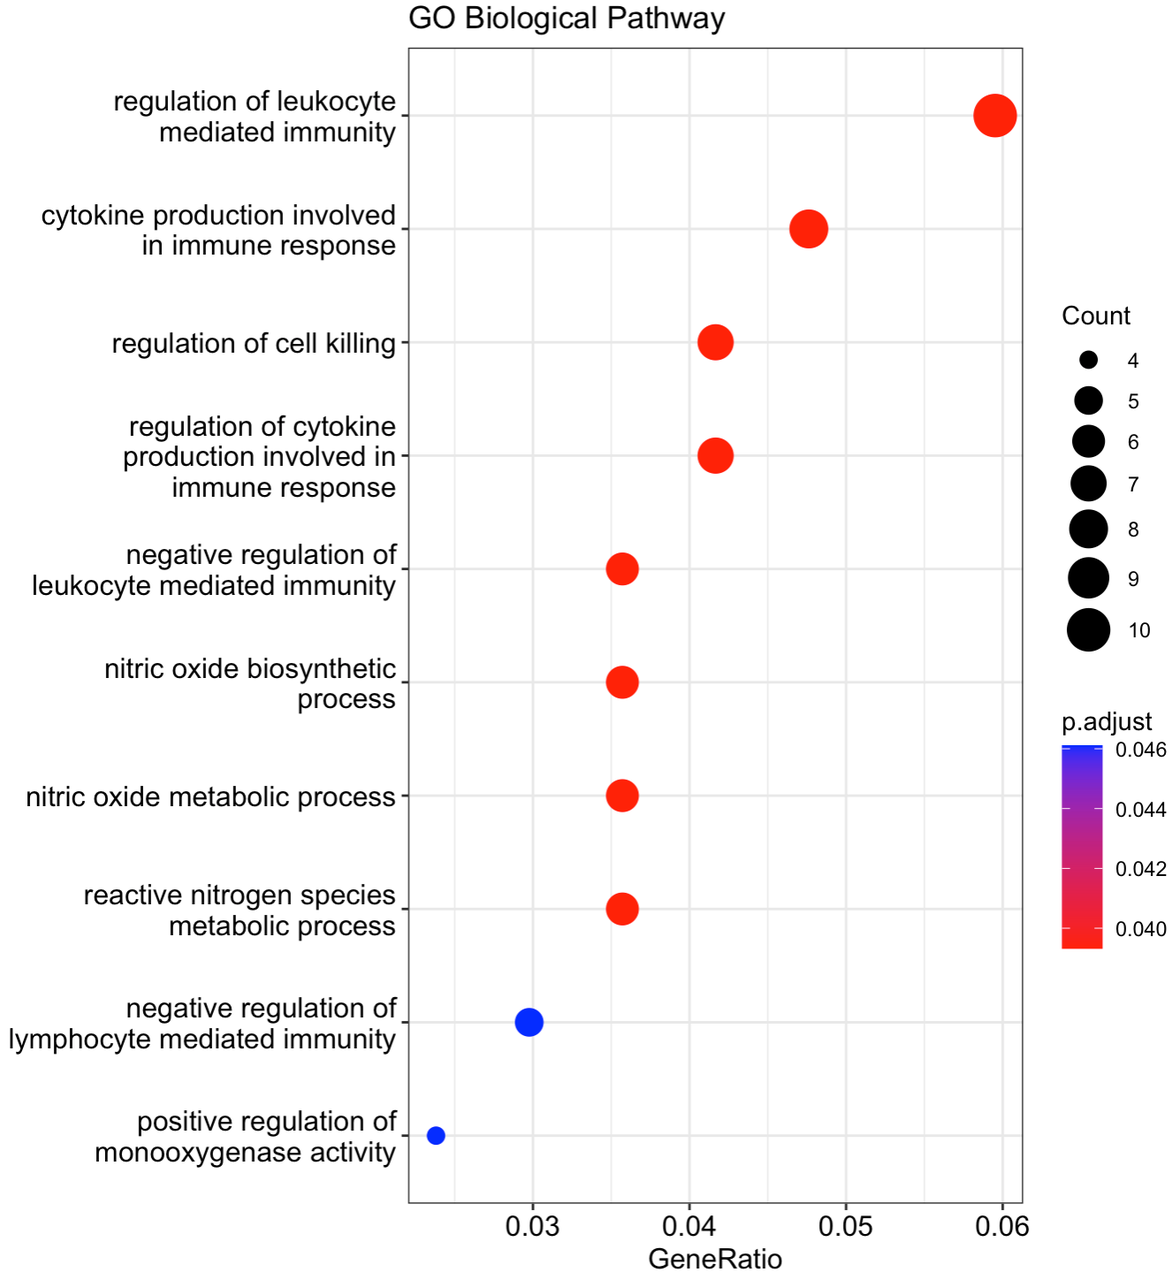
\includegraphics[width=10cm]{image/rnaseq/go.png}
    \caption{GO富集分析结果}
    \label{go}
\end{figure}